\section{Natural Language Toolkit - Class Imbalance}
\label{subsection:nltk-class_imbalance}

It was observed that there was a class imbalance between the positive and negative samples. In this section, it will be investigated if over sampling the minority positive class or under sample the majority negative class affects the performance of the model. A compromise solution where the positive class is partially over sampled and the negative class is partially under sampled is also examined. More advanced methods for handling class imbalance such as cost based learners or the Synthetic Minority Over-sampling Technique (SMOTE) are not suitable for consideration at this time using the NLTK datasets. Although not strictly a class imbalance solution, sampling using the most frequently observed features is also explored.

\subsection{Majority Class Under Sampling}
Under sampling of the majority negative class was first to be explored. In all NLTK datasets the ratio of negative to positive classes is between 4:1 and 5:1. To determine how different negative class to positive class ratios affect the model performance, under sampling of the majority class at ratios of 3:1, 2:1 and 1:1 to the minority class will be examined.

To implement the desired ratios, the Python script described in Section \ref{subsection:nltk-initial_modelling} requires one minor change as shown in Listing \ref{lst:chapter5.2:snipet_01}. The file ids of the not bullying, or negative class, are read into the \verb|all_neg_ids| list. The order of the file ids are then shuffled and the required ratio is achieved by only taking multiples of the number of positive ids as required. In line 6 the ratio of negative to positive samples is 3:1. 

\begin{lstlisting}[caption={Adjust the postive to negative class ratio}, label=lst:chapter5.2:snipet_01]
# The questions not containing bullying are the negative tests
all_neg_ids = reader.fileids('not_bullying')

# Shuffle the file ids of the negative file
random.shuffle(all_neg_ids)
neg_ids = all_neg_ids[:len(pos_ids)*3]
\end{lstlisting}

The NLTK Naive Bayes model was generated five times for each dataset and average performance values calculated. Because the negative samples are randomly chosen, it was important to run multiple executions for each dataset to allow for any possible variance or imbalance in the samples selected. It was found that five executions were enough to show that all results were similar and consistent. The performance results achieved for each dataset at ratios of 3:1, 2:1, 1:1, and the original performance measures from Section \ref{subsection:nltk-initial_modelling}, are shown in Figure \ref{fig:nltk_process_chart_03}.

\begin{figure}[htbp]
	\centering
	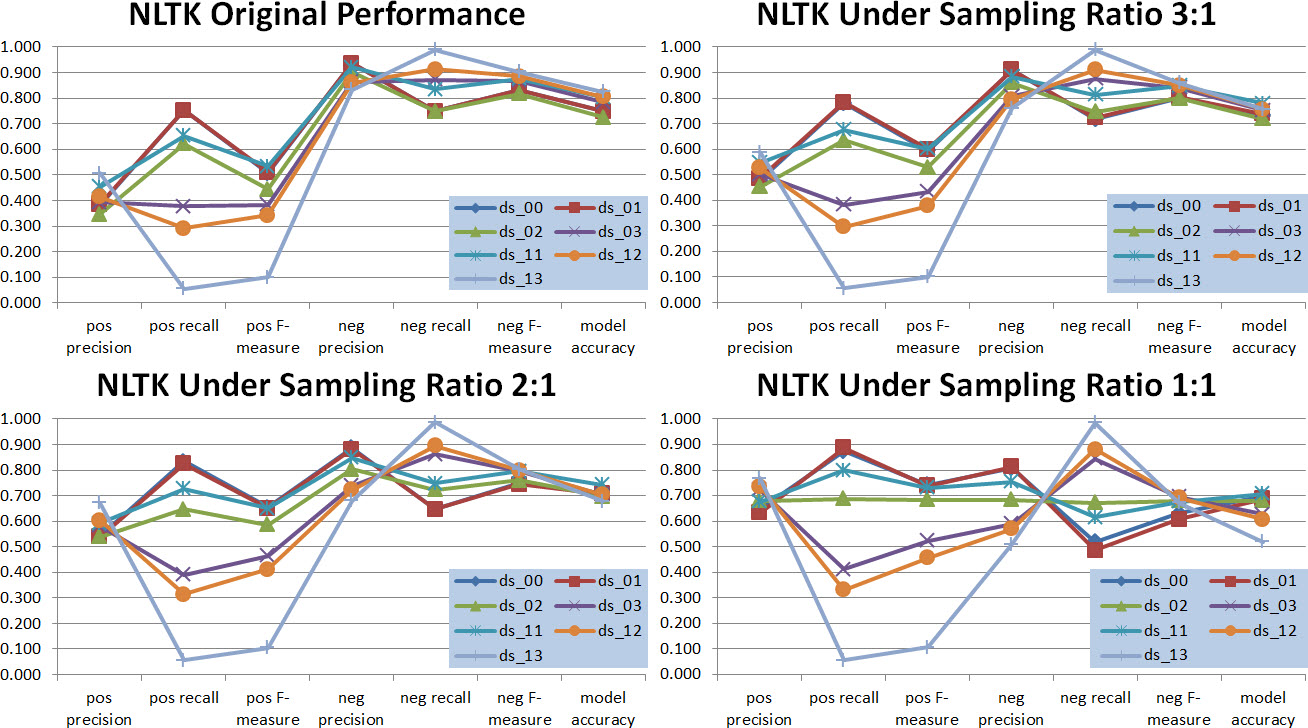
\includegraphics[width=1\textwidth]{Figures/Chapter5/nltk_process_chart_03.jpg}
	\caption[NLTK model performance using under sampling]{Graph showing the performance of the NLTK Naive Bayes model for ratios 3:1, 2:1, 1:1 and the original baseline performance measures}
	\label{fig:nltk_process_chart_03}
\end{figure}

It is clear that the performance of the positive class prediction is increasing as the ratio of samples approaches 1:1. The positive recall values for some of the datasets also show modest improvement, however, the values do not show the same improvement for \verb|dataset_03| tri-grams, \verb|dataset_12| bi-grams no stop words and \verb|dataset_13| tri-grams no stop words. This lack of improvement could be attributed to the uniqueness of the bi-grams and tri-grams in the datasets. It was seen in Section \ref{section:data_exploration} that the average frequency of n-grams in these datasets were very close to 1. Also of note is that as the ratio of classes approaches 1:1 the negative class precision and recall values are decreasing. 

At a ratio of 1:1 the overall performance of \verb|dataset_02|, bi-grams including stop words, could, at this early stage of development, be considered very satisfactory. With performance values in all categories of just under 70\% the model is equally accurate predicting both positive and negative classes. If the ability to solely predict the positive class was the main driving force, than both uni-grams models, with a sample ratio of 1:1, offer a better solution but at the cost of over predicting samples as positive. It must be kept in mind that one of the major drawbacks of under sampling in this manner is the risk of discarding samples that may, in fact, be very representative of the general population.

\subsection{Minority Class Over Sampling}
Over sampling of the positive minority class was explored next. Ratios of 3:1, 2:1 and 1:1 were again simulated, but this time, instead of reducing the number of negative samples in order to achieve these ratios the number of positive samples was increased. In line with all testing to this point the method used to increase the number of positive samples was as simple as possible. The implementation, in Python, is shown in Listing \ref{lst:chapter5.2:snipet_02} where a ratio of 2:1 is created.

\begin{lstlisting}[caption={Adjust the postive to negative class ratio}, label=lst:chapter5.2:snipet_02]
# The questions containing bullying are the positive tests
all_pos_ids = reader.fileids('bullying')
random.shuffle(all_pos_ids)

# Ratio 2:1 required
multi = (len(neg_ids)/2) / len(all_pos_ids)
modul = (len(neg_ids)/2) % len(all_pos_ids)

pos_ids = []

for n in range(multi):
    pos_ids = pos_ids + all_pos_ids

pos_ids = pos_ids + all_pos_ids[:modul]
\end{lstlisting}

When under sampling the negative class was randomly shuffled. This time the positive class is shuffled and the number of times the positive samples need to be replicated, to achieve the desired ratio, is calculated in lines 6 and 7. Taking \verb|dataset_13|, 1049 positive sample and 4915 negative, as an example, the number of times the full set of negative samples need to be replicated is $ ((4915/2) / 1049) = 2$. Then using the modulo operator the number of additional samples required is calculated $ ((4915/2) \% 1049) = 359$. So to create the test dataset two complete copies of the positive samples are required and additional 359 samples. As before, the model was generated five time to ensure that an average performance was achieved. Figure \ref{fig:nltk_process_chart_04} compares the performance results from the models generated using under sampling of the majority class with the models generated using over sampling.

\begin{figure}[htbp]
	\centering
	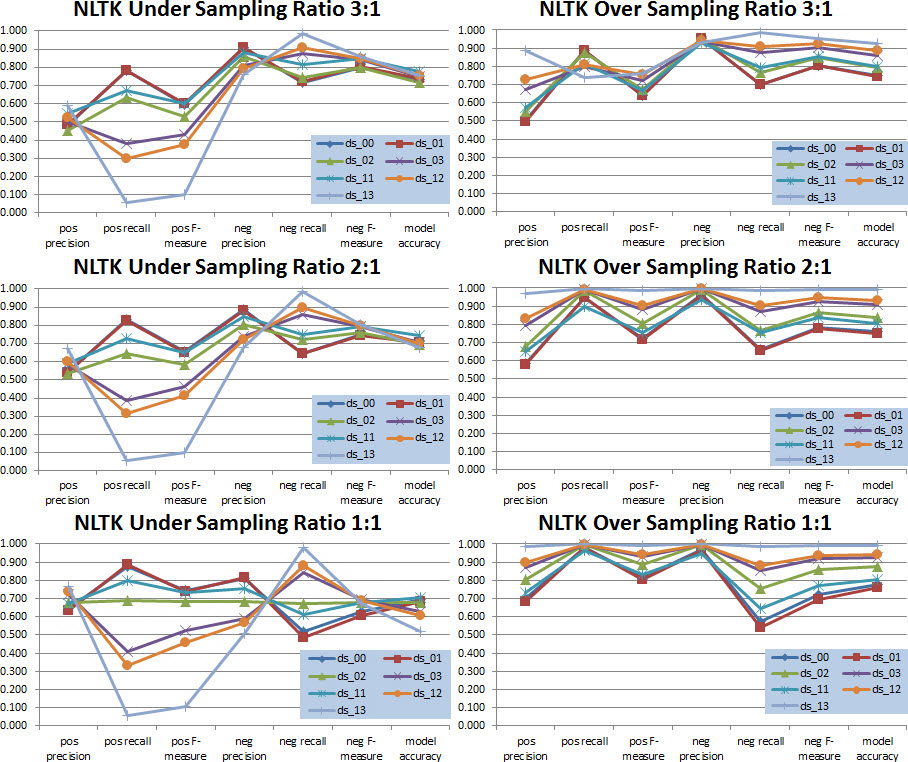
\includegraphics[width=1\textwidth]{Figures/Chapter5/nltk_process_chart_04.jpg}
	\caption[NLTK model performance using over sampling]{Graph showing the performance of the NLTK Naive Bayes model for over sampling ratios of 3:1, 2:1, 1:1 and the original baseline performance measures}
	\label{fig:nltk_process_chart_04}
\end{figure}

It is clear that over sampling of the minority positive class has significantly improved the performance of all models. Bi-gram and tri-gram tokens, with stop words removed, nearly achieving perfection with 99.8\% and 100\% positive sample recall and 88.4\% and 98.4\% negative sample recall respectively. Inversely though, it was also observed that as the ratio of the classes approaches 1:1 that the recall performance of the model predicting the negative class decreased significantly, particularly for all the uni-gram datasets.

Overall though, the results achieved using over sampling of the minority class outperform the models developed using under sampling of the majority class. It must be questioned though whether this gain in performance has been achieved by over fitting the models to the repeated samples? This over fitting to replicated data is a known issue when over sampling is applied.

\subsection{Hybrid Approach}
The third option used to tackle the imbalance of the positive and negative classes was a hybrid approach that uses both under sampling of the majority class and over sampling of the minority class. In this hybrid method, the normal approach is to take the total number of examples and then divide by the number of classes to get the target sample number. For example, in a two class scenario with 800 positive and 400 negative samples, the target number of samples for each class would be 600 if a ratio of 50:50 was the desired ratio. In this section, both classes are over or under sampled to half the total number of examples as just described. However, as the negative class is significantly superior to the negative sample, ratios of 60:40 and 70:30 are also explored. The additional python to achieve the required ratio of samples is shown in Listing \ref{lst:chapter5.2:snipet_03}.

\begin{lstlisting}[caption={Hybrid approach using both over and under sampling}, label=lst:chapter5.2:snipet_03]
# Calculate the number of pos and neg samples
pos_sample = int(float((len(all_neg_ids) + len(all_pos_ids)))
                 * 0.4)
neg_sample = int(float((len(all_neg_ids) + len(all_pos_ids)))
                 * 0.6)
# Ratio 50:50 required
multi_pos = pos_sample / len(all_pos_ids)
modul_pos = pos_sample % len(all_pos_ids)

modul_neg = neg_sample % len(all_neg_ids)
\end{lstlisting}

In this model both the positive file ids and the negative file ids are shuffled, not shown, and Listing \ref{lst:chapter5.2:snipet_03} lines 2 to 4 shows how the total number of positive and negative samples are calculated, in this case to a ratio of 60:40. The same sampling technique using \verb|modul| and \verb|multi|, as used in the over sampling model, is used to generate the sample datasets. As the negative class will never be over sampled only the \verb|modul| value needs to be calculated. Figure \ref{fig:nltk_process_chart_05} shows the result of the model execution using the hybrid sampling ratios.

\begin{figure}[htbp]
	\centering
	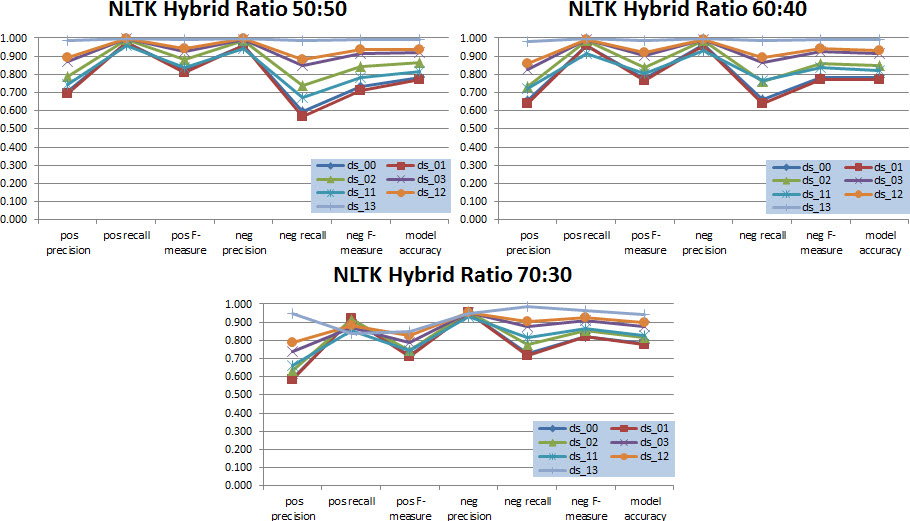
\includegraphics[width=1\textwidth]{Figures/Chapter5/nltk_process_chart_05.jpg}
	\caption[NLTK model performance using hybrid sampling]{Graph showing the performance of the NLTK Naive Bayes model for hybrid sampling ratios of 50:50, 60:40 and 70:30}
	\label{fig:nltk_process_chart_05}
\end{figure}

Comparing Figures \ref{fig:nltk_process_chart_04} and \ref{fig:nltk_process_chart_05} it is clear that the results achieved by over sampling to ratios of 1:1 and 2:1 are very similar to the results achieved by the 50:50 and 60:40 hybrid approach. This fact is highlighted by Table \ref{tab:chapter5:performance_comparison}. The top part of this table gives the results for the over sampling model where a ratio of 1:1 was used. The middle part of the table gives the performance results for the model where hybrid sampling with a ratio of 50:50 was used. The bottom part of the table gives the percentage change between the oversampling model and the hybrid sampling model. Excluding run time measurement, the majority of all performance measures between the two models are within 1\% of each other. Considering all performance measures, again excluding run time, then the total average performance difference between all the models of each type is just 0.18\%. Although the difference between the 2:1 over sampling model and the 60:40 hybrid model is slightly more obvious again the total average difference between the two models is just 1.78\%.

The final thing to consider is the run time. On average, the hybrid model is approximately 35\% faster. This is a significant time saving considering that the performance of the models are so similar. This variance in run time can be explained by the difference in the dataset sizes used. The over sampling dataset had, on average, just over 14,000 samples whereas the hybrid sampling dataset had an average size of just over 8,500. In this direct comparison of two models the obvious choice would be the hybrid approach. This difference in execution time could be pivotal is selecting the best models.

\begin{table}[h]
\centering
\caption[Performance comparison of over sampling and hybrid sampling]{Table giving the performance measured for over sampling at ratio 1:1 and hybrid sampling at 50:50 and the percentage differences}
\label{tab:chapter5:performance_comparison}
\begin{tabular}{rccccccc}
	\toprule
	\multicolumn{4}{c}{\textbf{Over Sampling Ratio 1:1}} \\
	\cmidrule(r){1-4}
     & \textbf{ds\_00}  & \textbf{ds\_01} & \textbf{ds\_02} & \textbf{ds\_03} & \textbf{ds\_11} & \textbf{ds\_12} & \textbf{ds\_13}   \\
    \midrule
	pos precision & 0.698 & 0.682 & 0.804 & 0.872 & 0.733 & 0.896 & 0.984\\
	pos recall & 0.981 & 0.981 & 0.997 & 0.998 & 0.965 & 0.998 & 1.000\\
	pos F-measure & 0.815 & 0.804 & 0.890 & 0.930 & 0.833 & 0.944 & 0.992\\
	neg precision & 0.968 & 0.966 & 0.996 & 0.998 & 0.949 & 0.997 & 1.000\\
	neg recall & 0.574 & 0.542 & 0.756 & 0.853 & 0.647 & 0.884 & 0.984\\
	neg F-measure & 0.720 & 0.693 & 0.859 & 0.919 & 0.769 & 0.937 & 0.992\\
	model accuracy & 0.777 & 0.761 & 0.876 & 0.925 & 0.806 & 0.941 & 0.992\\
	run time & 17.538 & 16.376 & 24.878 & 27.112 & 14.181 & 18.385 & 14.658\\
    \bottomrule
\end{tabular}
\begin{tabular}{rccccccc}
	\multicolumn{4}{c}{\textbf{Hybrid Sampling Ratio 50:50}} \\
	\cmidrule(r){1-4}
     & \textbf{ds\_00}  & \textbf{ds\_01} & \textbf{ds\_02} & \textbf{ds\_03} & \textbf{ds\_11} & \textbf{ds\_12} & \textbf{ds\_13}   \\
	\midrule
	pos precision & 0.707 & 0.692 & 0.791 & 0.870 & 0.744 & 0.894 & 0.984 \\
	pos recall & 0.975 & 0.975 & 0.992 & 0.995 & 0.957 & 0.996 & 1.000 \\
	pos F-measure & 0.819 & 0.809 & 0.880 & 0.928 & 0.837 & 0.942 & 0.992 \\
	neg precision & 0.959 & 0.957 & 0.989 & 0.994 & 0.940 & 0.996 & 1.000 \\
	neg recall & 0.595 & 0.566 & 0.737 & 0.850 & 0.670 & 0.881 & 0.984 \\
	neg F-measure & 0.734 & 0.711 & 0.844 & 0.917 & 0.782 & 0.935 & 0.992 \\
	model accuracy & 0.785 & 0.770 & 0.864 & 0.923 & 0.813 & 0.939 & 0.992 \\
	run time & 11.036 & 10.405 & 16.327 & 18.245 & 9.040 & 11.817 & 9.325 \\
	\bottomrule
\end{tabular}
\begin{tabular}{rccccccc}
	\multicolumn{4}{c}{\textbf{Percentage Difference}} \\
	\cmidrule(r){1-4}
     & \textbf{ds\_00}  & \textbf{ds\_01} & \textbf{ds\_02} & \textbf{ds\_03} & \textbf{ds\_11} & \textbf{ds\_12} & \textbf{ds\_13}   \\
	\midrule
	pos precision & 1.28 & 1.49 & -1.64 & -0.23 & 1.51 & -0.24 & 0 \\
	pos recall & -0.64 & -0.64 & -0.51 & -0.30 & -0.83 & -0.13 & 0 \\
	pos F-measure & 0.49 & 0.61 & -1.14 & -0.26 & 0.49 & -0.19 & 0 \\
	neg precision & -0.89 & -0.90 & -0.69 & -0.34 & -0.93 & -0.15 & 0 \\
	neg recall & 3.71 & 4.47 & -2.55 & -0.26 & 3.51 & -0.31 & 0 \\
	neg F-measure & 2.04 & 2.53 & -1.76 & -0.30 & 1.69 & -0.24 & 0 \\
	model accuracy & 0.96 & 1.18 & -1.39 & -0.28 & 0.91 & -0.21 & 0 \\
	run time & -37.07 & -36.46 & -34.37 & -32.70 & -36.25 & -35.72 & -36.38 \\
	\bottomrule
\end{tabular}
\end{table}

\subsection{Most Frequently Occurring Features}
Where over and under sampling tackles the class imbalance problem by attempting to equalise the number of positive and negative samples, another approach that was explored was to determine if the class imbalance problem could be solved by feature selection. Using a frequency distribution of all positive and negative tokens, the top \textit{x\%} most frequently occurring tokens in each class are chosen. Alternatively, choosing the same top \textit{n} positive and negative samples is also an option.

To achieve this feature sampling required significant changes to the original NLTK Python script described in Section \ref{subsection:nltk-initial_modelling}. A partial listing of the Python Script, where it is different from the original script, is given in Appendix \ref{app:nltk_feature_selection}. The highlights are shown in Listing \ref{lst:chapter5.2:snipet_04} where the additional functionality required to extract to most frequently tokens for the positive class is shown.

The first difference is that the list of all words for the positive class is generated, lines 5 to 8. Next the frequency distribution is created and the top percentage is extracted. In line 12 the top 25\% most frequently occurring tokens are chosen and the comment in line 13 shows how the top 500 tokens would be chosen. Finally, the dictionary describing whether the top features are present or not in the samples is created. As shown in lines 1 to 3 this function is slightly different in that it is checked whether each token is one of the top tokens and, if it is, only then is it included as a feature.

\begin{lstlisting}[caption={Selecting the most frequently occuring tokens}, label=lst:chapter5.2:snipet_04]
def pos_word_feats(words):
    return dict([(word, True) for word in words
                 if word in top_pw])

pos_words = []

for fileid in pos_ids:
    pos_words += [word for word in (reader.words(fileid))]

pw_dist =  nltk.FreqDist(pos_words)

top_pw = pw_dist.keys()[:int(len(pw_dist.keys())*.25)]
# top_pw = pw_dist.keys()[:500]

pos_feat = [(pos_word_feats(reader.words(fileids=[f])),
             'bullying')
            for f in pos_ids]
\end{lstlisting}

The performance measures returned using the most frequently occurring tokens was very disappointing and they did not show any improvement over the baseline from Section \ref{subsection:nltk-initial_modelling}. Feature selection combined with over, under and hybrid sampling actually returned worse performance measures than the sampling techniques did on their own.  